\documentclass{beamer}
\usetheme{AnnArbor}
\usepackage{graphicx}
% Figures live one level up in ../figures relative to this .tex file
% Search both ../ (so includegraphics{figures/...} works) and ../figures/ (so includegraphics{...} works)
\graphicspath{{../}{../figures/}}
\usepackage{amsmath}
\usepackage{amssymb}
\usepackage{framed}
\usepackage{tikz}
\usepackage[]{xcolor}
\usepackage[most]{tcolorbox}
\usepackage{pgfplots}
\pgfplotsset{compat=1.18}
\usepackage{blkarray}
\setbeamercolor{mycolorbox}{%
  bg=yellow!20,   % background color (20% yellow)
  fg=black      % foreground (text) color
}
\usefonttheme[onlymath]{serif}

\newtcolorbox{solutionblock}{
  colback=yellow!5,        % Background color: light yellow
  colframe=orange!80!black, % Frame color: dark orange
  title=Solution,
  fonttitle=\bfseries
}

\title{Introduction to Functions}
\author{Nithin}
\institute{}
\date{\today}
\begin{document}
\begin{frame}
  \titlepage
\end{frame}
\begin{frame}
  \tableofcontents
\end{frame}
\section{Slopes and Average Rate of Change}

% Slide: Motivation and Overview
\begin{frame}{Motivation: Why Study Change?}
  \begin{itemize}
    \item Calculus explores how quantities change and provides tools for modeling these changes.
    \item Functions link inputs ($x$) to outputs ($y=f(x)$); we investigate how $y$ varies as $x$ moves over an interval.
    \item Real-world example: Predicting economic indicators, modeling speeds, and more.
  \end{itemize}
\end{frame}

% Slide: Defining Average Rate of Change
\begin{frame}{Average Rate of Change}
  \begin{block}{Definition}
    For a function $f(x)$ on interval $[a,b]$, the \emph{average rate of change} is
    \[ 
      \frac{f(b)-f(a)}{b-a},
    \]
    which geometrically represents the slope of the secant line between $(a,f(a))$ and $(b,f(b))$.
  \end{block}
  \begin{itemize}
    \item Rise: $f(b)-f(a)$
    \item Run: $b-a$
    \item Secant line smooths out fluctuations; reports overall trend.
  \end{itemize}
\end{frame}

% Slide: Graphical Illustration
\begin{frame}{Graphical Illustration}
  \begin{columns}
    \column{0.6\textwidth}
      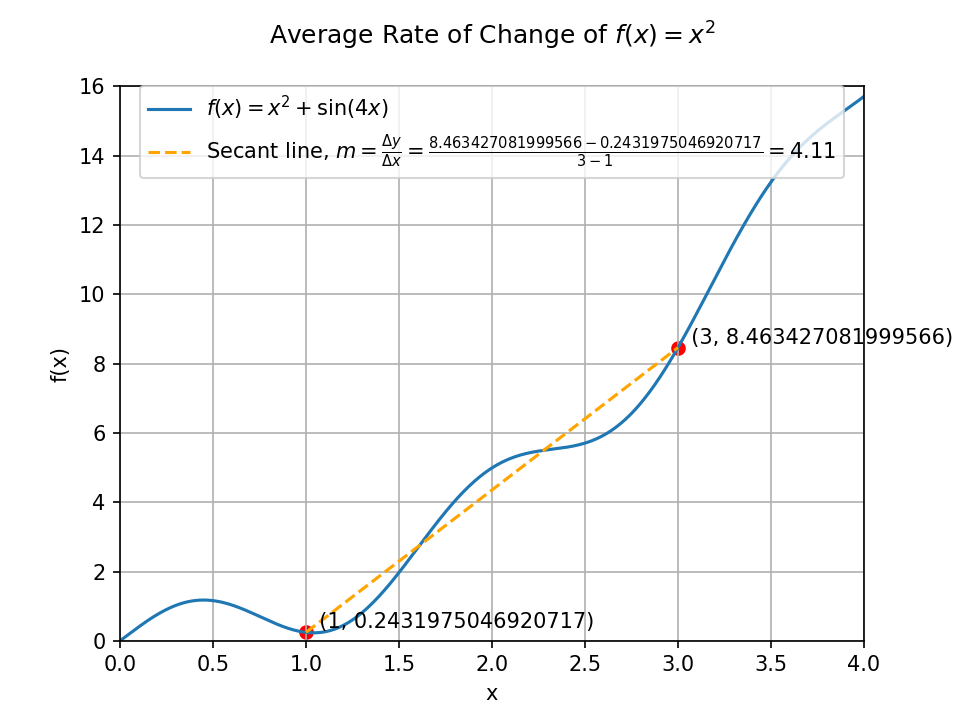
\includegraphics[width=\textwidth]{figures/avg_rate_of_change.png}
    \column{0.4\textwidth}
      \begin{itemize}
        \item Focus on interval $[1,3]$ on the curve $y=f(x)$.
        \item Secant line (in orange) joins $(1,f(1))$ and $(3,f(3))$.
        \item Its slope measures the average change in $y$ per unit change in $x$.
      \end{itemize}
  \end{columns}
\end{frame}

% Slide: Problem – Trivandrum to Chennai Average Speed
\begin{frame}{Example: Trivandrum to Chennai Journey}
  \begin{columns}
    \column{0.5\textwidth}
      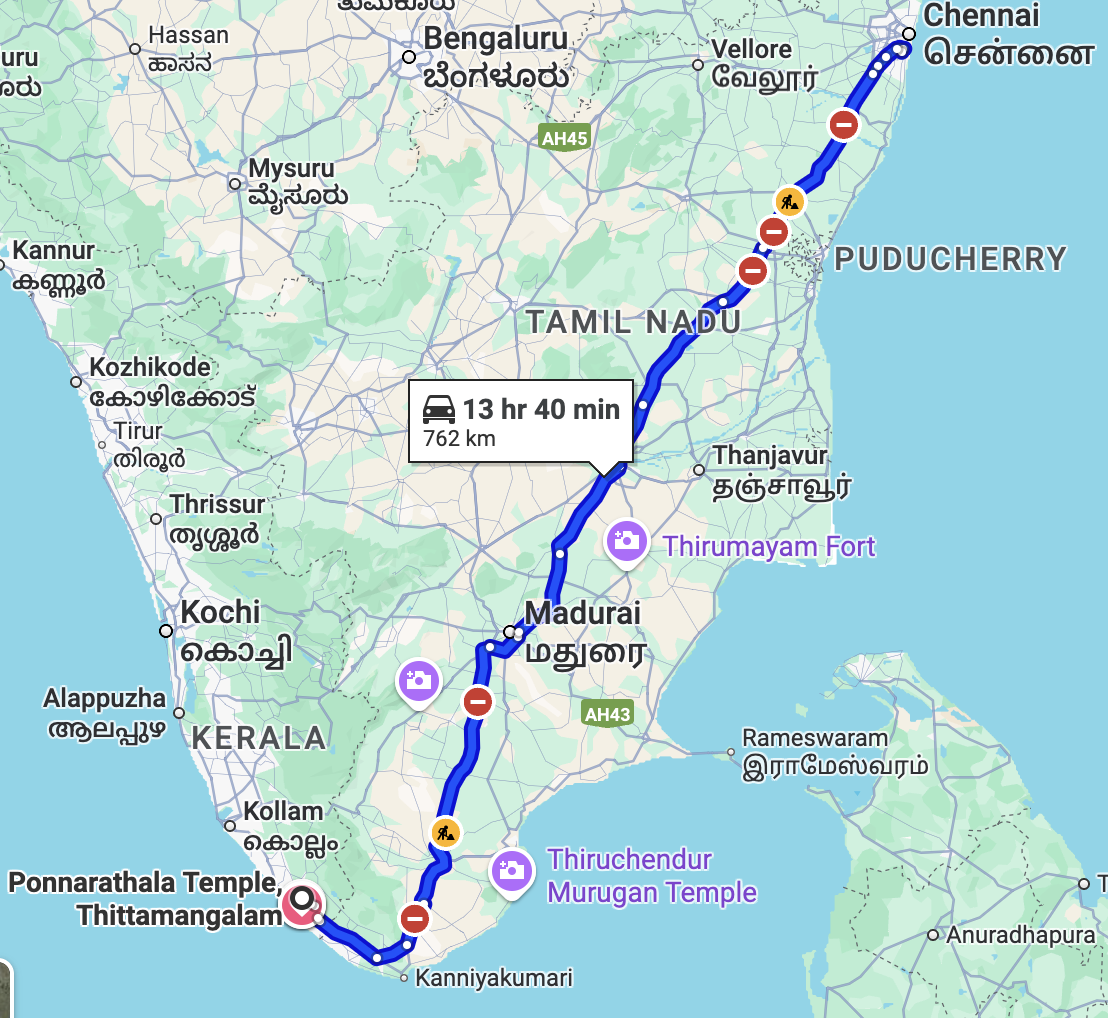
\includegraphics[width=\textwidth]{figures/trivandrum_chennai_map.png}
    \column{0.5\textwidth}
      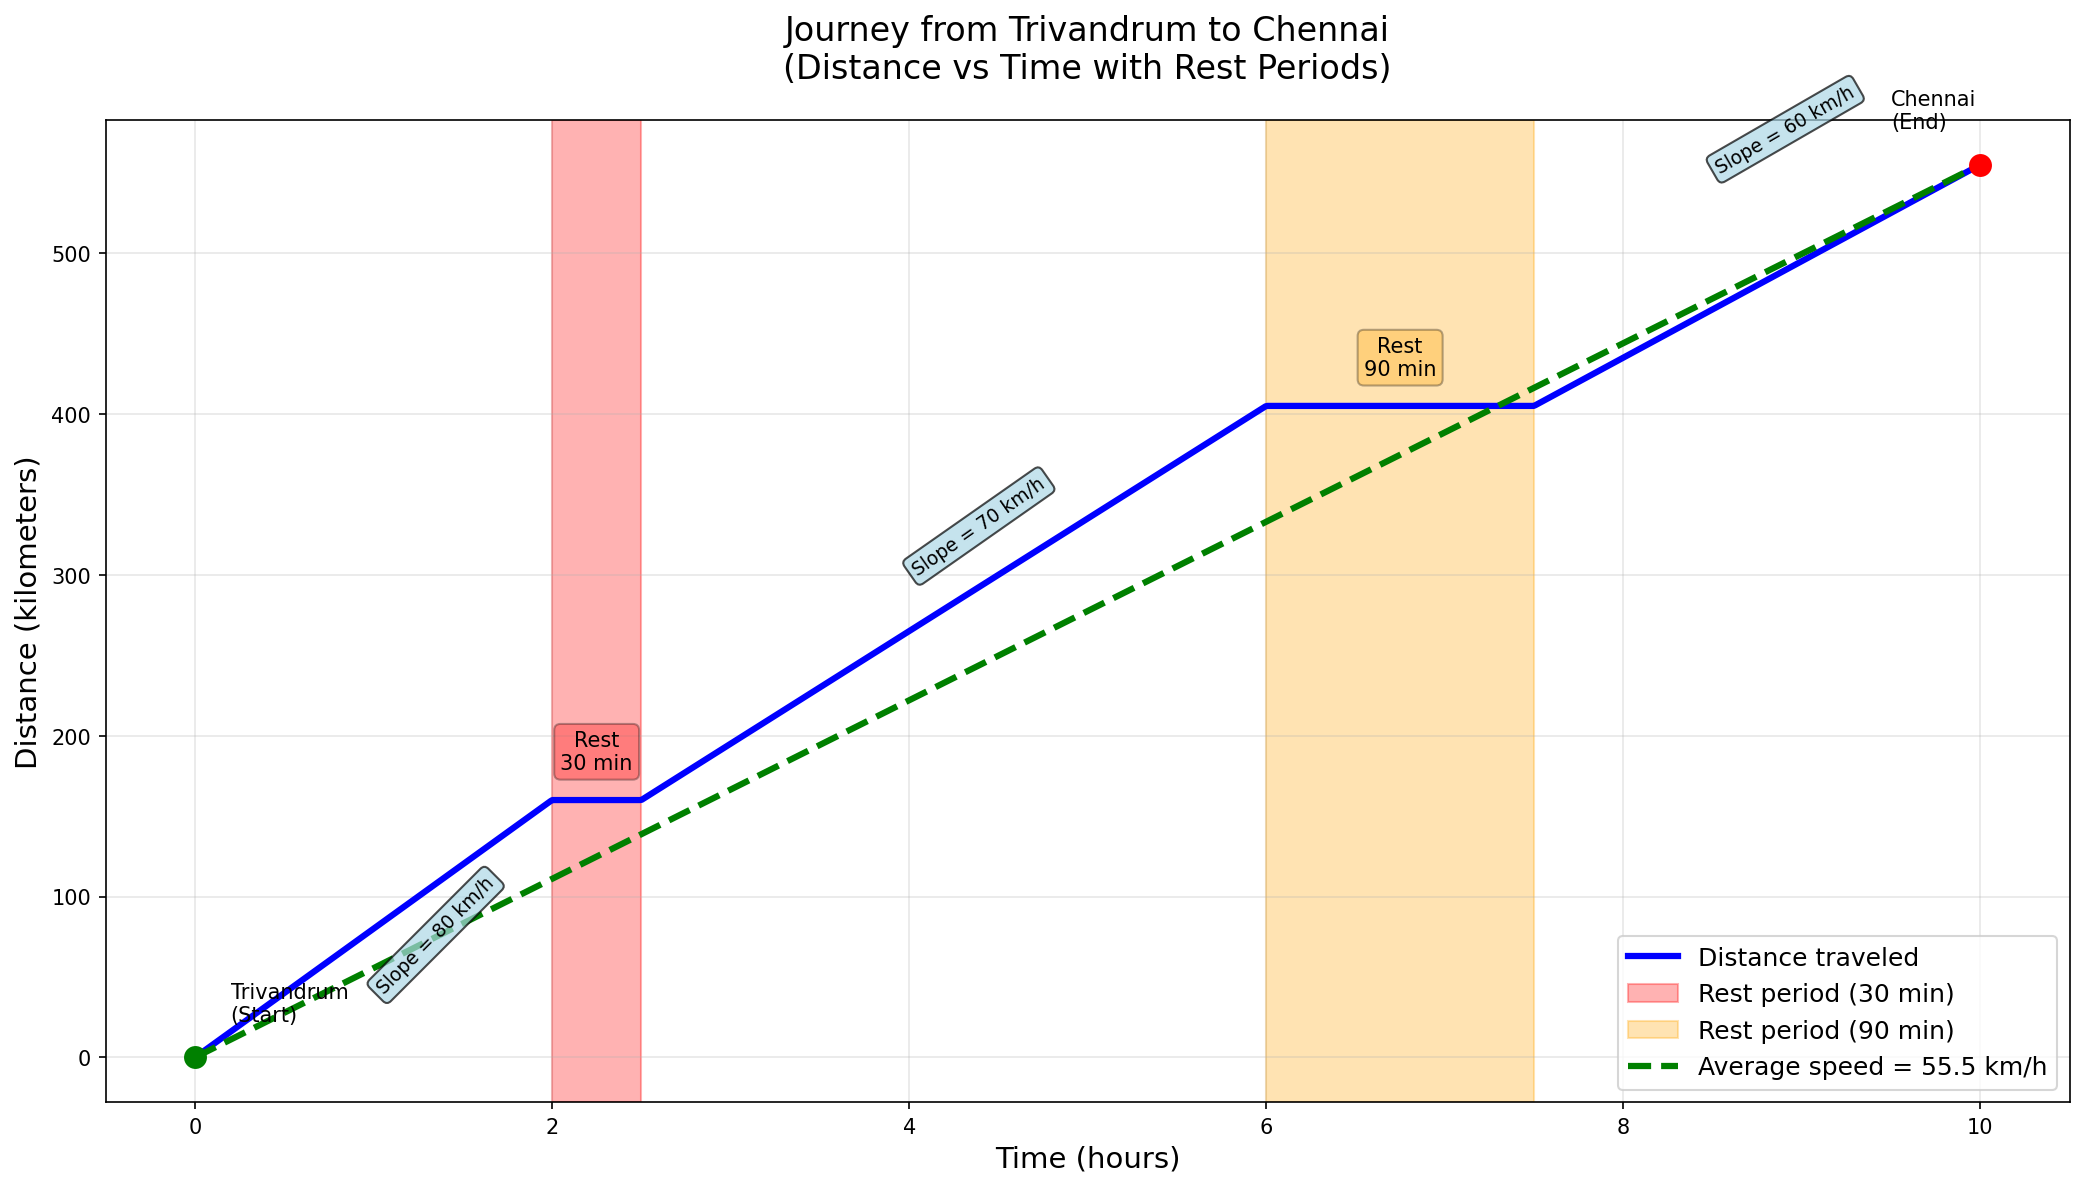
\includegraphics[width=\textwidth]{figures/trivandrum_chennai_journey.png}
  \end{columns}
  \vspace{1ex}

\end{frame}

\begin{frame}
  \begin{itemize}
    \item Total distance: 762 km
    \item Total time (including stops): 15 hours
    \item Average speed: $\dfrac{762}{15}\approx50.8$ km/h
  \end{itemize}
  \begin{solutionblock}
    Average speed $=\dfrac{\text{distance}}{\text{time}}=\dfrac{762}{15}\approx50.8\text{ km/h}$.  
  This illustrates how the secant slope over an interval gives overall performance even with rest periods.
  \end{solutionblock}
\end{frame}

\begin{frame}
\frametitle{Why Instantaneous Rate of Change?}
\begin{itemize}
  \item Average rate of change provides overall performance but lacks detail.
  \item Instantaneous rate of change captures behavior at a specific moment while average rate is over an interval
  \item Essential for understanding dynamic systems (e.g., velocity, acceleration).
  \item Instantaneous rate of change = calculate average rathe of change over smaller and smaller intervals.
\end{itemize}
\end{frame}
\begin{frame}{Graphical Illustration: Instantaneous Rate of Change}
  \centering
  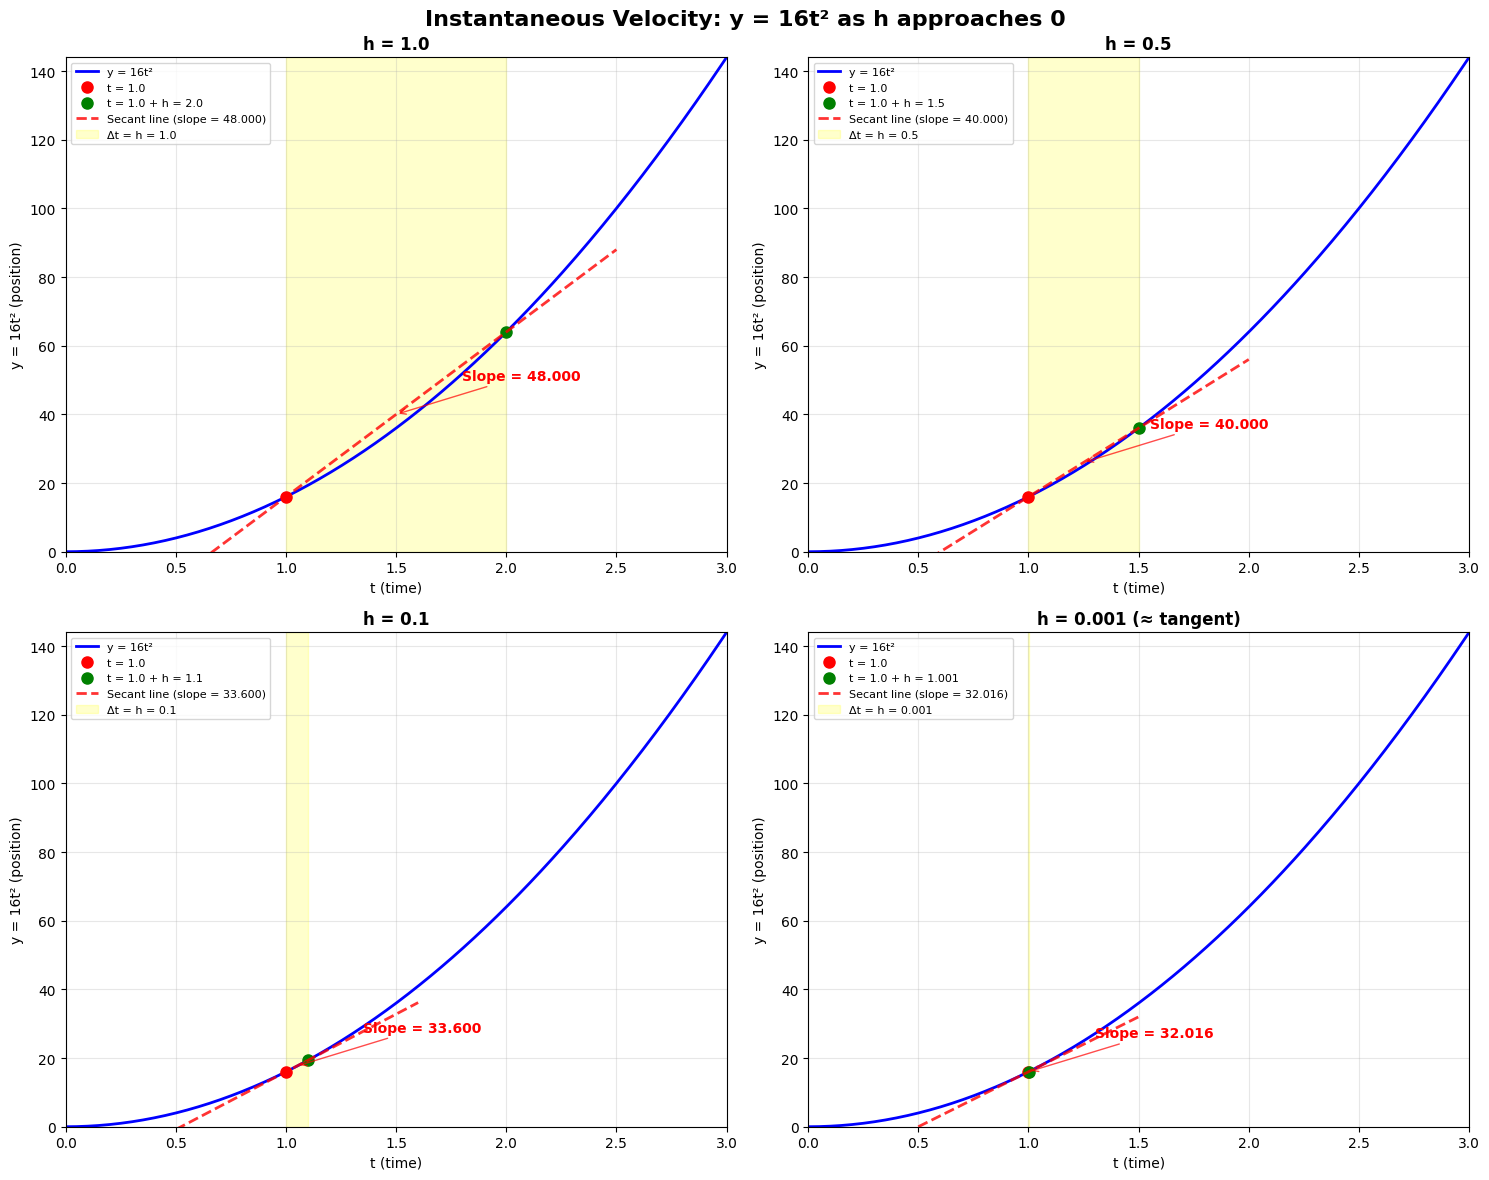
\includegraphics[width=0.8\textwidth]{figures/instantaneous_rate_change.png}
\end{frame}

% Slide: Toward Instantaneous Rate of Change
\begin{frame}{Instantaneous Rate of Change}
  \begin{itemize}
    \item Instantaneous speed corresponds to slope of tangent line at a point.
    \item As secant interval shrinks ($b\to a$), average rate approaches derivative $f'(x)$.
    \item Next: Formalize tangent lines and derivatives.
  \end{itemize}
\end{frame}

\begin{frame}
  \frametitle{The Mean Value Theorem}
  \begin{figure}
    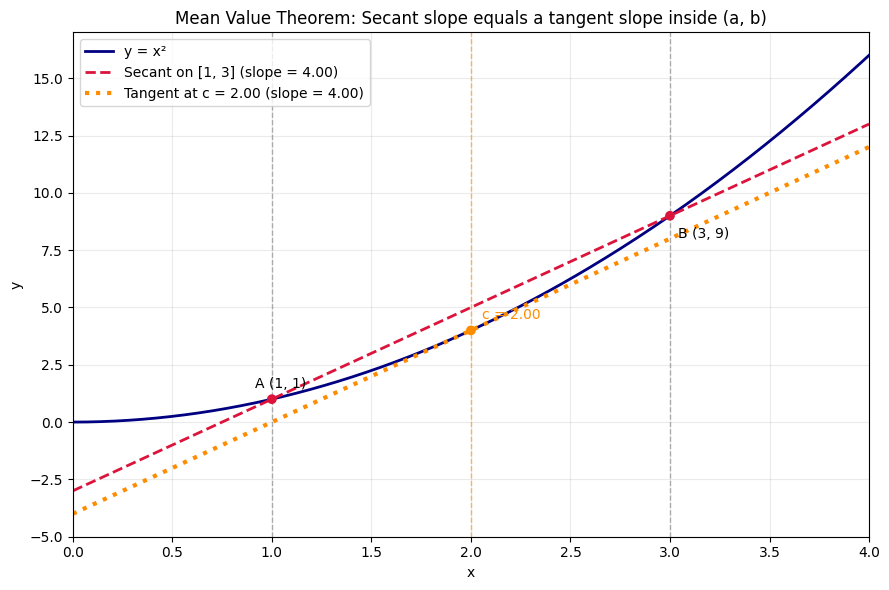
\includegraphics[width=0.75\textwidth]{figures/mean_value.png}
    \caption{Mean Value Theorem: There exists a point $c$ where the tangent equals the secant.}
  \end{figure}
\end{frame}
% Slide: Mean Value Theorem (informal, no derivatives)
\begin{frame}{The Mean Value Theorem (informal, no derivatives)}
  \begin{block}{Statement}
  For a smooth curve $y=f(x)$ on an interval $[a,b]$, the \emph{average rate of change}
  \[ \dfrac{f(b)-f(a)}{b-a} \]
  is realized as the slope of a \emph{tangent line} at some point $x=c$ with $a<c<b$.
  In other words, the secant line joining $(a,f(a))$ and $(b,f(b))$ has the same slope as
  the tangent line to the curve at some point inside the interval.
  \end{block}
  \vspace{0.5em}
\end{frame}
\section{Displacement, Velocity, and Acceleration}
\begin{frame}{Displacement}
  \begin{block}{Definition}
    The displacement $x(t)$ at time $t$ measures position on the real line relative to an origin $0$, so positive values indicate one direction and negative values the opposite.
  \end{block}
  \begin{itemize}
    \item Independent variable: time $t$ (typically seconds).
    \item Dependent variable: displacement $x$.
    \item Choice of origin and direction provides a signed measure of position.
  \end{itemize}
\end{frame}

\begin{frame}{Velocity}
  \begin{block}{Definition}
    The velocity $v(t)$ is the instantaneous rate of change of displacement $x(t)$.
  \end{block}
  \begin{itemize}
    \item $v(t)>0$ (motion in the positive direction), $v(t)<0$ (negative direction), or $v(t)=0$.
    \item Speed is the magnitude of velocity: $\text{speed}=\lvert v(t)\rvert$.
    \item A speedometer displays instantaneous speed.
  \end{itemize}
\end{frame}

\begin{frame}{Acceleration}
  \begin{block}{Definition}
    The acceleration $a(t)$ is the instantaneous rate of change of velocity $v(t)$.
  \end{block}
  \begin{itemize}
    \item $a(t)$ may be positive, negative, or zero.
    \item The term “deceleration” is often used when $a(t)$ is negative and quoted as a positive number by convention.
  \end{itemize}
\end{frame}

\begin{frame}{Example: Cannonball Projectile}
  \begin{figure}
    \centering
    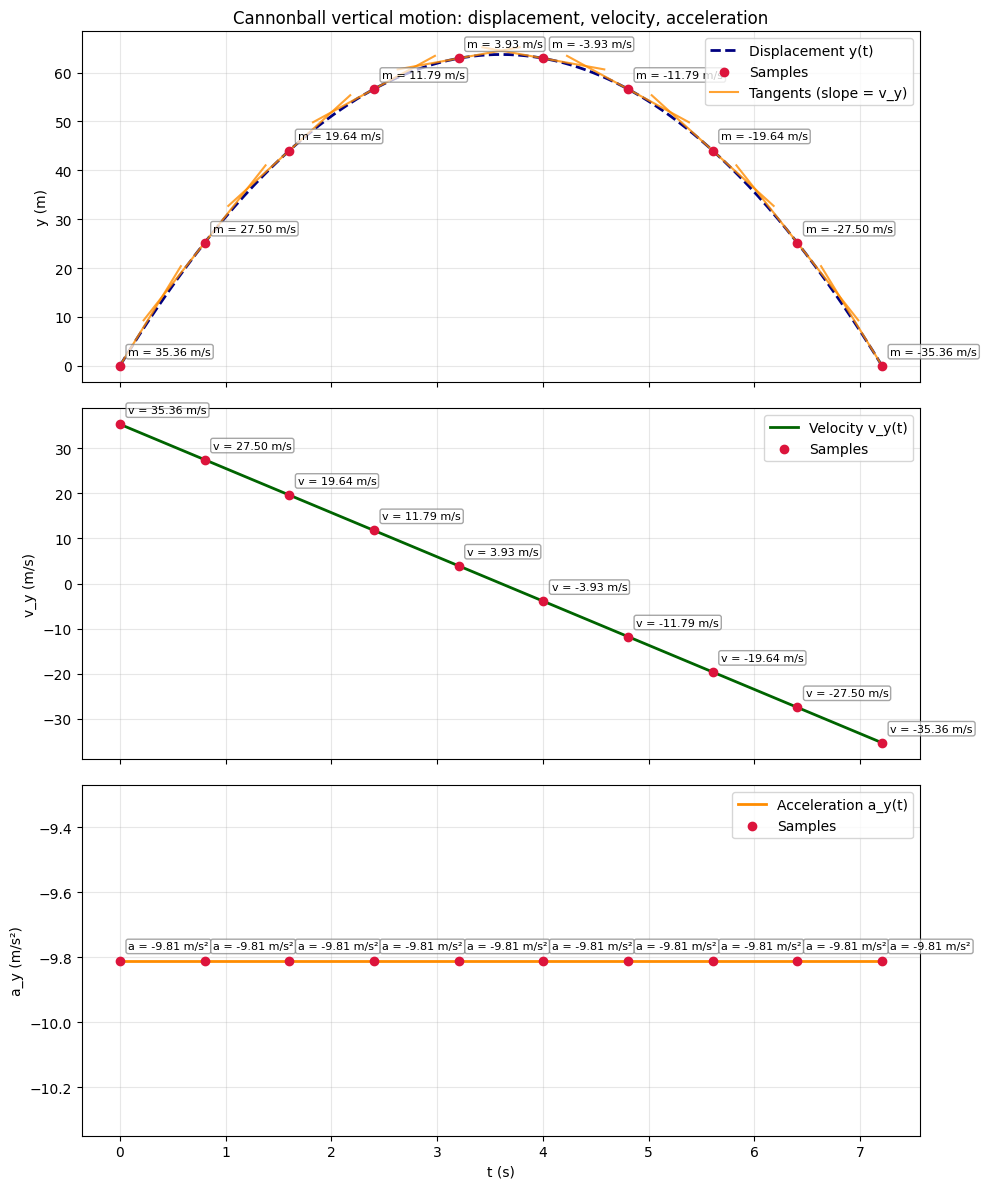
\includegraphics[width=0.5\textwidth]{figures/cannonball.png}
  \end{figure}
\end{frame}

\end{document}